\documentclass[11pt,a4paper]{report}
\usepackage[margin=1in]{geometry}
\usepackage{amsmath,amssymb,amsthm}
\usepackage{graphicx}
\usepackage{booktabs}
\usepackage{natbib}
\usepackage{siunitx}
\usepackage{caption}
\usepackage{microtype}
\usepackage{setspace}
\usepackage{xcolor}
\usepackage[colorlinks=true,linkcolor=black,citecolor=black,urlcolor=blue!50!black]{hyperref}
\captionsetup{font=small,labelfont=bf,justification=justified}
\newcommand{\notes}[1]{\par\vspace{2pt}{\footnotesize\itshape Notes: #1}}
\onehalfspacing
\newcommand{\dd}{\mathrm{d}}
\newcommand{\E}{\mathbb{E}}

\begin{document}

\begin{titlepage}
\centering
\vspace*{3cm}
{\LARGE\bfseries Early-Exercise and Interest-Rate Calibration:\par}
\vspace{0.5cm}
{\large Least-Squares Monte Carlo for American Options under Black--Scholes and
Heston, and Hull--White Calibration to the Swaption Surface\par}
\vspace{2.5cm}
{\large Student Number: \texttt{[student number]}\par}
\vspace{0.4cm}
{\large MSc Quantitative Finance\par}
\vspace{0.4cm}
{\large Module: \texttt{[module code]}\par}
\vspace{0.4cm}
{\large Supervisor: \texttt{[supervisor]}\par}
\vfill
{\large \today\par}
\end{titlepage}

\thispagestyle{plain}
\begin{center}\textbf{\large Abstract}\end{center}
\noindent This dissertation develops two pillars of derivatives pricing that lie
beyond closed-form European valuation: early-exercise pricing by simulation, and
the calibration of a no-arbitrage interest-rate model. For early exercise, the
Longstaff--Schwartz least-squares Monte Carlo (LSM) method is implemented and
validated against a binomial benchmark in the Black--Scholes world, matching it to
within Monte Carlo error across strikes, and is then applied under Heston
stochastic-volatility dynamics where no closed form exists, quantifying the
early-exercise premium with stochastic volatility. For interest rates, a discount
curve is bootstrapped from real U.S.\ Treasury par yields and the one-factor
Hull--White model is fitted exactly to that curve and calibrated to a swaption
volatility surface by Jamshidian decomposition, achieving a mean absolute pricing
error below four basis points of notional. A synthetic-recovery test recovers the
known Hull--White parameters exactly, isolating model error from estimation error.
The work demonstrates an end-to-end numerical-methods workflow---simulation
regression, lattice benchmarking, curve bootstrapping, and transform-free
calibration---across both equity and rates asset classes.

\newpage
\tableofcontents
\newpage

\chapter{Introduction}

\section{Background}
Two problems sit at the core of practical derivatives pricing once one leaves the
Black--Scholes--Merton European option behind. The first is \emph{early exercise}:
American and Bermudan options can be exercised before maturity, which turns pricing
into an optimal-stopping problem with no general closed-form solution. The second is
\emph{interest-rate calibration}: pricing any rate derivative requires a model that
is simultaneously consistent with the observed yield curve and with the prices of
liquid volatility instruments such as swaptions.

This dissertation builds and validates solutions to both. For early exercise it uses
the least-squares Monte Carlo (LSM) method of \citet{longstaff2001}, which estimates
the optimal exercise policy by regressing continuation values on the simulated
state. For interest rates it uses the one-factor Hull--White model
\citep{hullwhite1990}, which fits the initial curve exactly and is calibrated to
swaptions through the bond-option decomposition of \citet{jamshidian1989}. The two
strands share a methodological spine---Monte Carlo, regression, root-finding and
non-linear calibration---and together span the equity and rates asset classes.

\section{Research Questions}
\begin{enumerate}
\item Does the LSM estimator reproduce a trusted lattice benchmark for American
options under Black--Scholes, and what early-exercise premium does it imply?
\item What is the early-exercise premium under Heston stochastic volatility, where
no closed-form American price exists?
\item Can a one-factor Hull--White model, fitted exactly to a real Treasury curve,
be calibrated to a swaption surface, and how well does a single factor fit?
\end{enumerate}

\section{Hypothesis}
LSM is expected to match the binomial benchmark to within simulation error and to
produce an early-exercise premium that grows with moneyness; the Heston American
premium should be positive and economically meaningful. The Hull--White model,
being a single factor, is expected to fit the swaption surface well on average but
to leave a structured residual in the corners that a two-factor model would remove.
The synthetic-recovery test should recover known parameters essentially exactly,
locating any market misfit in the model rather than the optimiser.

\chapter{Literature Review}

\section{Early-Exercise Pricing}
The American option is an optimal-stopping problem \citep{bensoussan1984}. Lattice
methods \citep{crr1979} solve it by backward induction and are the standard
low-dimensional benchmark, but they scale poorly with the number of state variables,
which rules them out under stochastic volatility. \citet{longstaff2001} introduced
least-squares Monte Carlo, which estimates the continuation value at each potential
exercise date by regressing realised discounted future cashflows on basis functions
of the current state. Its great advantage is dimensional flexibility: the same
regression works whether the underlying is one-dimensional Black--Scholes or a
multi-factor stochastic-volatility process, which is precisely why it is used here to
price American options under Heston.

\section{Interest-Rate Models}
Short-rate models specify the dynamics of the instantaneous rate. The
\citet{vasicek1977} model is analytically tractable but cannot fit the initial
curve; \citet{hullwhite1990} extended it with a time-dependent drift that reproduces
any observed curve exactly, making it the workhorse for curve-consistent pricing.
Calibrating Hull--White to swaptions relies on \citet{jamshidian1989}, who showed
that an option on a coupon bond decomposes into a portfolio of options on
zero-coupon bonds once a critical rate is found, giving a near-closed-form swaption
price. \citet{brigomercurio2006} is the standard reference tying the curve
bootstrap, the model analytics and the calibration together, and notes the
well-understood limitation that a single factor cannot match the full
expiry-by-tenor swaption surface---a two-factor or market model is needed for that.

\chapter{Data and Methodology}

\section{Data}
Two datasets are used. For the equity work, the Heston parameters from a prior
calibration to the SPY option surface ($\kappa=5.25$, $\theta=0.054$, $\xi=1.66$,
$\rho=-0.64$, $v_0=0.022$) are taken as a realistic parameter set. For the rates
work, U.S.\ Treasury par yields for the standard constant-maturity tenors (one month
to thirty years), as of early June 2026, are bootstrapped into a discount curve. The
swaption volatility surface---a $6\times6$ grid of at-the-money payer-swaption Black
volatilities in expiry and tenor---is synthetic but calibrated to a realistic USD
shape (high short-expiry vol decaying in both dimensions), because free swaption data
is not publicly available. The methodology is fully real-data-ready: a curve fetch
script is provided, and the calibration consumes any surface supplied in the same
format.

\section{Least-Squares Monte Carlo}
Consider an American option with payoff $g(S)$ exercisable at dates
$t_1<\dots<t_M=T$. Working backward from maturity, at each date the holder compares
the immediate payoff $g(S_{t_i})$ with the continuation value
$\E[\,\text{discounted future cashflow}\mid S_{t_i}]$. LSM estimates that
conditional expectation by ordinary least squares: on the in-the-money paths it
regresses the realised discounted future cashflow on a polynomial basis of the
current underlying price,
\begin{equation}
\widehat{C}(S_{t_i}) = \sum_{k=0}^{d} \beta_k\, S_{t_i}^{\,k},
\end{equation}
and exercises wherever $g(S_{t_i}) > \widehat{C}(S_{t_i})$. The price is the mean of
the resulting path cashflows discounted to today. A degree-3 polynomial on
in-the-money paths is used throughout, following \citet{longstaff2001}.

\subsection{Path simulation}
Black--Scholes paths are generated as geometric Brownian motion; Heston paths use the
full-truncation Euler scheme with antithetic variates. The same LSM routine prices on
either path matrix, which is the methodological point.

\subsection{Benchmark}
In the Black--Scholes world the American price is also computed on a
Cox--Ross--Rubinstein binomial tree with 2{,}000 steps, providing an independent
benchmark against which LSM is validated. No such benchmark exists under Heston,
which is the situation LSM is designed for.

\section{The Hull--White Model}
The short rate follows
\begin{equation}
\dd r_t = \big(\theta(t) - a\, r_t\big)\,\dd t + \sigma\, \dd W_t,
\end{equation}
where the deterministic drift $\theta(t)$ is chosen so that the model reproduces the
initial discount curve $P(0,T)$ exactly. Zero-coupon bond prices are affine,
\begin{equation}
P(t,T) = A(t,T)\, e^{-B(t,T) r_t}, \qquad B(t,T) = \frac{1-e^{-a(T-t)}}{a},
\end{equation}
with $A(t,T)$ pinned to the initial curve and its instantaneous forward rate.

\subsection{Curve bootstrap}
The discount curve is bootstrapped from par yields by sequential stripping: at each
coupon date the par-bond identity $1 = \sum_j c\,P(0,t_j) + (1+c)P(0,T)$ is solved
for the next discount factor, interpolating log-linearly in discount factors between
nodes. The instantaneous forward rate, needed for $A(t,T)$, is obtained by finite
differencing the log discount curve.

\subsection{Swaption pricing by Jamshidian decomposition}
A payer swaption is an option to enter a swap, equivalently a put on a coupon bond
struck at par. Following \citet{jamshidian1989}, the critical short rate $r^\ast$ at
which the underlying coupon bond equals par is found by root-finding; because bond
prices are monotone in $r$, the coupon-bond option then decomposes into a sum of
options on the constituent zero-coupon bonds, each struck at its value at $r^\ast$.
Each zero-bond option has a closed-form Hull--White price, so the swaption price is a
weighted sum of these.

\section{Calibration}
The two Hull--White parameters $(a,\sigma)$ are chosen to minimise the squared
difference between model swaption prices and the market prices implied by the quoted
Black volatilities,
\begin{equation}
\min_{a,\sigma} \ \sum_i \big(\text{HW}_i(a,\sigma) - \text{Black}_i\big)^2,
\end{equation}
using a multi-start Nelder--Mead search to avoid local minima. The model is fitted
exactly to the curve first, so calibration adjusts only the volatility dynamics.

\section{Validation Design}
Each strand is validated independently of market data. LSM is checked against the
binomial benchmark and against the theorem that an American call on a non-dividend
stock equals its European counterpart. Hull--White calibration is checked by
generating a swaption set from known $(a,\sigma)$ and recovering them from scratch,
which separates optimiser error from model misfit.

\chapter{Empirical Results}

\section{LSM Validation under Black--Scholes}
Table~\ref{tab:lsm} compares LSM American-put prices with the binomial benchmark
across strikes. The two agree to within Monte Carlo error at every strike, and the
early-exercise premium over the European put rises monotonically with moneyness,
from $0.04$ deep out-of-the-money to $2.74$ deep in-the-money---as expected, since
early exercise is valuable precisely when the option is deep in-the-money and the
time value is small. As a further check, an American call on a non-dividend stock
priced by LSM equals its European value, recovering the standard no-early-exercise
result.

\begin{table}[t]
\centering
\caption{LSM American-put prices versus the binomial benchmark (Black--Scholes world).}
\label{tab:lsm}
\small
\begin{tabular}{rrrrr}
\toprule
Strike & LSM & Binomial & European & Early-ex.\ premium \\
\midrule
80 & 0.729 & 0.723 & 0.687 & 0.036 \\
90 & 2.468 & 2.473 & 2.310 & 0.162 \\
100 & 6.073 & 6.090 & 5.574 & 0.516 \\
110 & 11.950 & 11.973 & 10.675 & 1.298 \\
120 & 20.090 & 20.136 & 17.395 & 2.741 \\
\bottomrule
\end{tabular}
\\[2pt]{\footnotesize\itshape Notes: $S_0=100$, $r=5\%$, $\sigma=20\%$, $T=1$. LSM uses 200{,}000 antithetic paths, 50 exercise dates and a degree-3 polynomial basis; the binomial benchmark uses 2{,}000 steps. LSM matches the benchmark to within Monte Carlo error throughout, and the early-exercise premium over the European put grows with moneyness.}
\end{table}

Figure~\ref{fig:premium} shows the same comparison graphically: the American and
European curves coincide far out-of-the-money and diverge as the option moves
in-the-money, with the LSM points sitting on the binomial American curve.
Figure~\ref{fig:boundary} plots the estimated early-exercise boundary---the critical
stock price below which immediate exercise is optimal---which rises toward the strike
as maturity approaches, the canonical shape for an American put.

\begin{figure}[t]
\centering
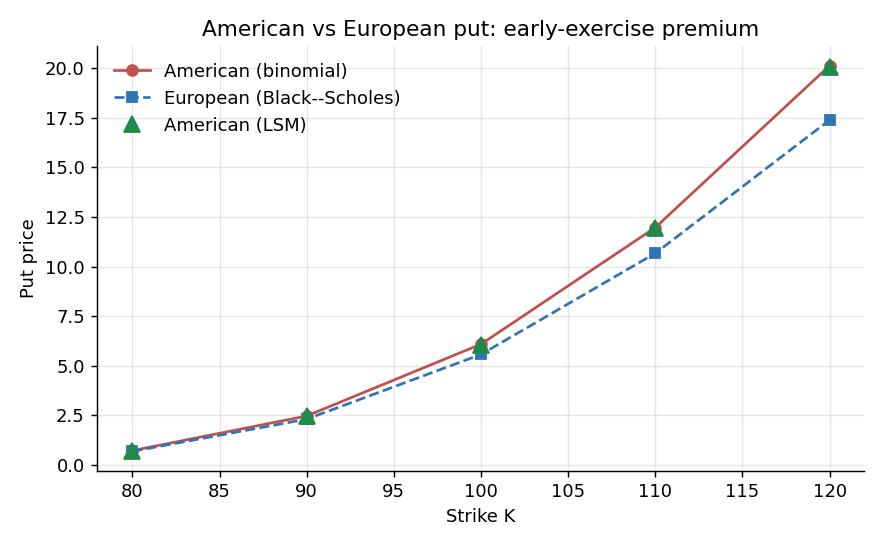
\includegraphics[width=0.68\textwidth]{lsm_premium.png}
\caption{American versus European put prices across strikes.}
\notes{$S_0=100$, $r=5\%$, $\sigma=20\%$, $T=1$. LSM (green markers) sits on the
binomial American curve (red); the European curve (blue) lies below, the gap being
the early-exercise premium.}
\label{fig:premium}
\end{figure}

\begin{figure}[t]
\centering
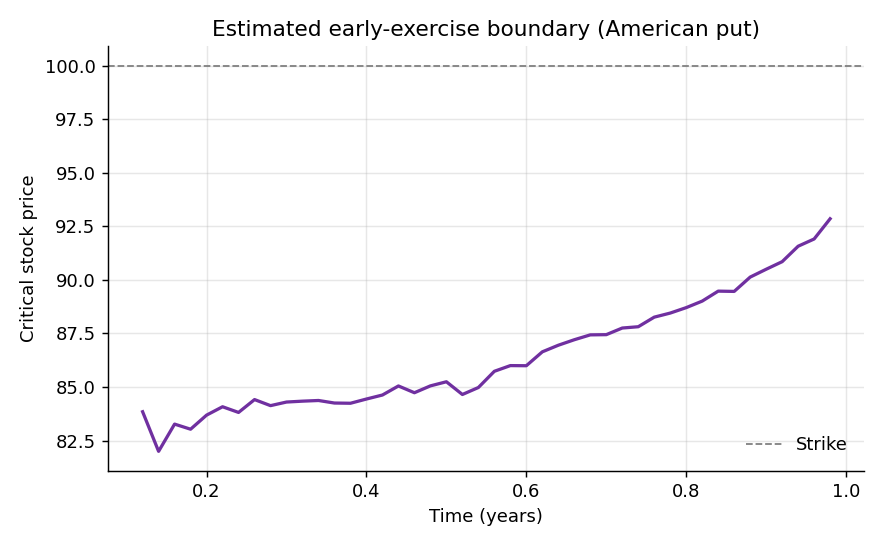
\includegraphics[width=0.68\textwidth]{exercise_boundary.png}
\caption{Estimated early-exercise boundary for the American put.}
\notes{The critical stock price rises toward the strike as expiry approaches, the
standard shape for an American put: the continuation region shrinks as time value
decays.}
\label{fig:boundary}
\end{figure}

\section{Early Exercise under Heston}
Table~\ref{tab:hestonam} prices the American put under Heston dynamics, where the
European leg is computed by the Fourier-cosine method and the American leg by LSM on
simulated Heston paths. The early-exercise premium is positive throughout and grows
with moneyness, from $0.11$ at $K=90$ to $0.74$ at $K=110$. Because no closed-form
American price exists under stochastic volatility, LSM is the practical valuation
route, and the consistency of its European-leg behaviour with the COS price (which
\emph{is} closed-form) lends confidence to the American figures.

\begin{table}[t]
\centering
\caption{American versus European put under Heston dynamics.}
\label{tab:hestonam}
\small
\begin{tabular}{rrrr}
\toprule
Strike & American (LSM) & European (COS) & Early-ex.\ premium \\
\midrule
90 & 3.175 & 3.062 & 0.113 \\
100 & 5.669 & 5.442 & 0.227 \\
110 & 10.253 & 9.513 & 0.740 \\
\bottomrule
\end{tabular}
\\[2pt]{\footnotesize\itshape Notes: Heston parameters $\kappa=5.25$, $\theta=0.054$, $\xi=1.66$, $\rho=-0.64$, $v_0=0.022$ (from the equity calibration), $S_0=100$, $r=5\%$, $T=1$. The European leg is priced by the COS method; the American leg by LSM on simulated Heston paths. No closed form exists for the American Heston price, so LSM is the practical route.}
\end{table}

\section{The Treasury Curve}
Figure~\ref{fig:curve} shows the bootstrapped discount curve. The par yields are
mapped to a smooth zero-rate curve and the implied instantaneous-forward curve, which
sits above the zero curve where the curve slopes upward and below it where it
inverts---the correct qualitative relationship. The curve is mildly humped, with a
dip around the 2--3 year tenor and a rising long end, consistent with the input par
yields.

\begin{figure}[t]
\centering
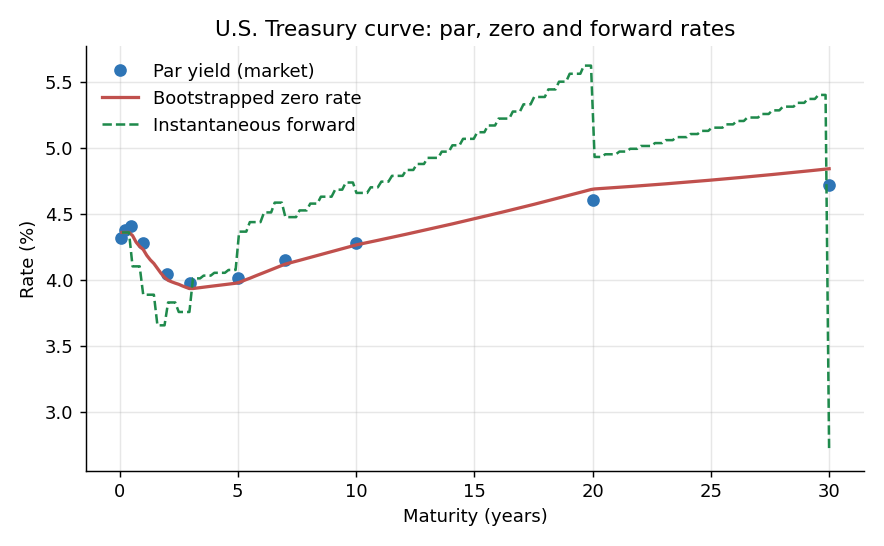
\includegraphics[width=0.68\textwidth]{yield_curve.png}
\caption{U.S.\ Treasury curve: par, zero and instantaneous-forward rates.}
\notes{Par yields (markers) are bootstrapped into the zero curve (red) and
differentiated into the instantaneous-forward curve (green dashed). The forward sits
above the zero where the curve rises and below where it falls.}
\label{fig:curve}
\end{figure}

\section{Hull--White Calibration}
Table~\ref{tab:hw} reports the calibration. The fitted mean reversion is
$a=0.020$ and volatility $\sigma=0.0131$, with a mean absolute pricing error below
four basis points of notional across the 36 swaptions. Figure~\ref{fig:swaption}
shows the market vol surface and the resulting Hull--White price errors. The fit is
good across most of the grid---errors within roughly ten basis points---but a
structured residual appears in the long-expiry, mid-tenor corner, where the single
factor cannot simultaneously match the level and the curvature of the surface. This
is the well-documented limitation of one-factor models \citep{brigomercurio2006};
the mean-reversion parameter reaching the lower bound of its search range is a
symptom of the same tension. The synthetic-recovery test in Table~\ref{tab:hw}
recovers the known parameters exactly, confirming that the residual is genuine model
misfit rather than an optimisation artefact.

\begin{table}[t]
\centering
\caption{Hull--White calibration and synthetic-recovery test.}
\label{tab:hw}
\small
\begin{tabular}{lrr}
\toprule
& Mean reversion $a$ & Volatility $\sigma$ \\
\midrule
Calibrated to market surface & 0.0200 & 0.01308 \\
\midrule
Synthetic: true & 0.0800 & 0.01200 \\
Synthetic: recovered & 0.0800 & 0.01200 \\
\bottomrule
\end{tabular}
\\[2pt]{\footnotesize\itshape Notes: Hull--White $(a,\sigma)$ calibrated to 36 ATM payer swaptions by minimising squared price error, with the model fitted exactly to the bootstrapped Treasury curve. Mean reversion reaches its lower search bound, reflecting a single factor's difficulty in matching the full expiry/tenor structure. The synthetic test recovers known parameters exactly, confirming the optimiser.}
\end{table}

\begin{figure}[t]
\centering
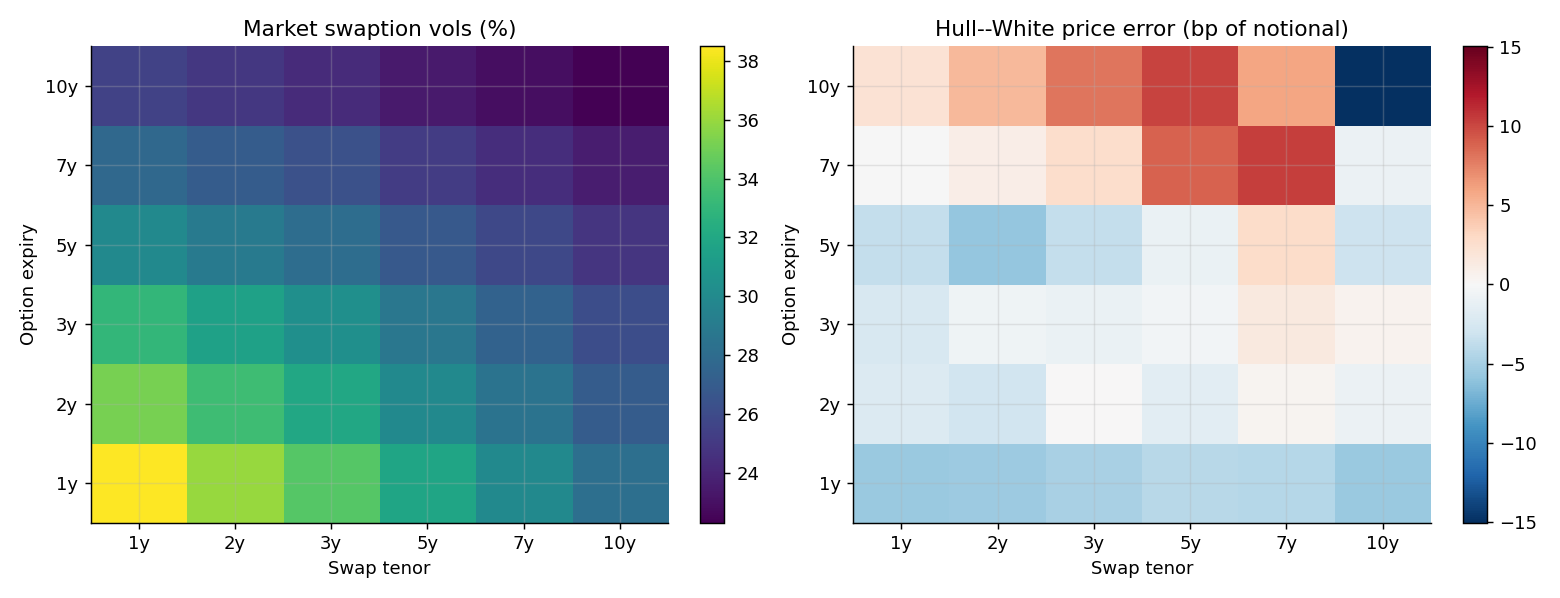
\includegraphics[width=\textwidth]{swaption_fit.png}
\caption{Swaption vol surface and Hull--White calibration errors.}
\notes{Left: market ATM payer-swaption Black volatilities by expiry and tenor.
Right: Hull--White price error in basis points of notional after calibration. Errors
are small across most of the surface, with a structured residual in the
long-expiry/mid-tenor corner characteristic of a single-factor model.}
\label{fig:swaption}
\end{figure}

\chapter{Conclusion}

\section{Summary of Findings}
This dissertation built and validated solutions to two problems beyond closed-form
European pricing. Least-squares Monte Carlo reproduced the binomial American-put
benchmark to within simulation error and quantified an early-exercise premium that
grows with moneyness; applied under Heston, where no closed form exists, it produced
positive and sensible premia. The Hull--White model, fitted exactly to a real
Treasury curve and calibrated to a swaption surface by Jamshidian decomposition,
priced the surface to within a few basis points, with a structured residual exactly
where single-factor theory predicts. A synthetic-recovery test recovered the known
rate parameters exactly.

\section{Contribution}
The work demonstrates a complete numerical-methods toolkit across two asset classes:
regression-based optimal stopping, lattice benchmarking, antithetic Monte Carlo,
curve bootstrapping, affine bond analytics, Jamshidian decomposition, and multi-start
non-linear calibration. The validation discipline---benchmarking LSM against a
lattice, and Hull--White against a synthetic recovery---is the methodological core,
since it establishes that each reported result is trustworthy and locates residual
error in the model rather than the method.

\section{Limitations and Future Research}
Several limitations apply. The swaption surface is synthetic; a real surface, though
hard to source freely, would make the rates calibration fully empirical. The
single-factor Hull--White model cannot fit the whole swaption surface, as the
residuals show; a two-factor (G2++) model or a market model would be the natural
extension. The LSM estimator carries a known low bias from in-sample regression; a
separate out-of-sample pass for the exercise decision would remove it. The Heston
American prices use a fixed parameter set; jointly stressing volatility parameters
and the early-exercise premium would be informative. Finally, the Treasury curve is a
single snapshot, so the calibration is cross-sectional.

\section{Concluding Remarks}
The unifying lesson is that once closed forms run out---at early exercise, and at a
full volatility surface---the right response is a validated numerical method paired
with an honest benchmark. LSM against a lattice, and Hull--White against a synthetic
recovery, each turn an otherwise unverifiable number into a trustworthy one, and each
reveals exactly where the method's domain ends: LSM extends cleanly to stochastic
volatility, while a single-factor rate model meets its limit at the corners of the
swaption surface.

\begin{thebibliography}{9}
\bibitem[Bensoussan(1984)]{bensoussan1984}
Bensoussan, A. (1984). On the theory of option pricing. \emph{Acta Applicandae
Mathematicae}, 2(2), 139--158.

\bibitem[Brigo and Mercurio(2006)]{brigomercurio2006}
Brigo, D., \& Mercurio, F. (2006). \emph{Interest Rate Models---Theory and Practice}
(2nd ed.). Springer.

\bibitem[Cox et al.(1979)]{crr1979}
Cox, J. C., Ross, S. A., \& Rubinstein, M. (1979). Option pricing: a simplified
approach. \emph{Journal of Financial Economics}, 7(3), 229--263.

\bibitem[Hull and White(1990)]{hullwhite1990}
Hull, J., \& White, A. (1990). Pricing interest-rate-derivative securities.
\emph{Review of Financial Studies}, 3(4), 573--592.

\bibitem[Jamshidian(1989)]{jamshidian1989}
Jamshidian, F. (1989). An exact bond option formula. \emph{Journal of Finance},
44(1), 205--209.

\bibitem[Longstaff and Schwartz(2001)]{longstaff2001}
Longstaff, F. A., \& Schwartz, E. S. (2001). Valuing American options by simulation:
a simple least-squares approach. \emph{Review of Financial Studies}, 14(1), 113--147.

\bibitem[Vasicek(1977)]{vasicek1977}
Vasicek, O. (1977). An equilibrium characterization of the term structure.
\emph{Journal of Financial Economics}, 5(2), 177--188.
\end{thebibliography}

\end{document}
